%%%%%%%%%%%%%%%%%%%%%%%%%%%%%%%%%%%%%%%%%%%%%%%%%%%%%%%%%%%%%%%%%%%%
\section{Interfaces (3 pages)} ~\label{sec:fdsp-apa-intfc}

%\fixme{It would be nice to coordinate with the interface documents; email to Jack F sent 12/20}

The interface between the APA consortium and other detector consortia, facilities, and working groups
covers a wide range activities. Table~\ref{tab:apa_interface_docdb} summarizes the interface control
documents being developed. In the following, we are going to elaborate on three relative important
interfaces: electronics, photon detector, and high voltage system. 

\begin{table}[!htp]
  \caption{Summary of interface control documents being developed.}  
\medskip
\renewcommand{\arraystretch}{1.1} \centering 
\begin{tabular}{|c|c|}
  \hline
  Name & DUNE doc-db number \\\hline
  Interface to TPC electronics & 6670 \\ 
  Interface to photon detector & 6667 \\
  Interface to joint high voltage & 6673 \\
  Interface to joint DAQ & 6676 \\
  Interface to joint slow controls and cryogenics infrastructure & 6679 \\\hline
  Integration facility Interface & 7021 \\
  Facility interfaces (Detector Hall, Cryostat, and Cryogenics) & 6967 \\
  Installation Interface & 6994 \\
  Calibration to Interface & 7048 \\\hline
  Software computing interface & 7102 \\
  Physics interface & 7075 \\\hline
\end{tabular}\label{tab:apa_interface_docdb}
\end{table}

\fixme{Include an image of each interface in appropriate section.}

%%%%%%%%%%%%%%%%%%%%%%%%%%%%%%%%%
\subsection{TPC Cold Electronics}~\label{sec:fdsp-apa-intfc-elec}

As shown in Fig.~\ref{fig:apa_ce}, all 2560 APA wires are terminated on the wire boards, which are stacked
along the electronics end (head) of the APA frame. Ten stacks of wire boards are installed across the width 
of each side of the head frame. There are a total of 128 (48, 40, 40, 48 wires from X, U, V, and G layer,
respectively) readout channels for each stack of wire board. The TPC readout electronics is directly
mounted on the APA immersed inside LAr, in order to reduce the input capacitance and thus the inherent
electronics noise. The 2560 channels is readout by 20 Front-End Motherboards (FEMBs), each of which includes
eight 16-channel Front End (FE) ASICs, eight 16-channel ADC ASICs, low-voltage regulators, and input signal 
protection circuits. 

\begin{dunefigure}[APA electronics interface]{fig:apa_ce}
{Zoom-in view of the head region of APA frame. 20  FEMBs together with the corresponding wire board (10 on each side) are shown. See text for more explanations.}
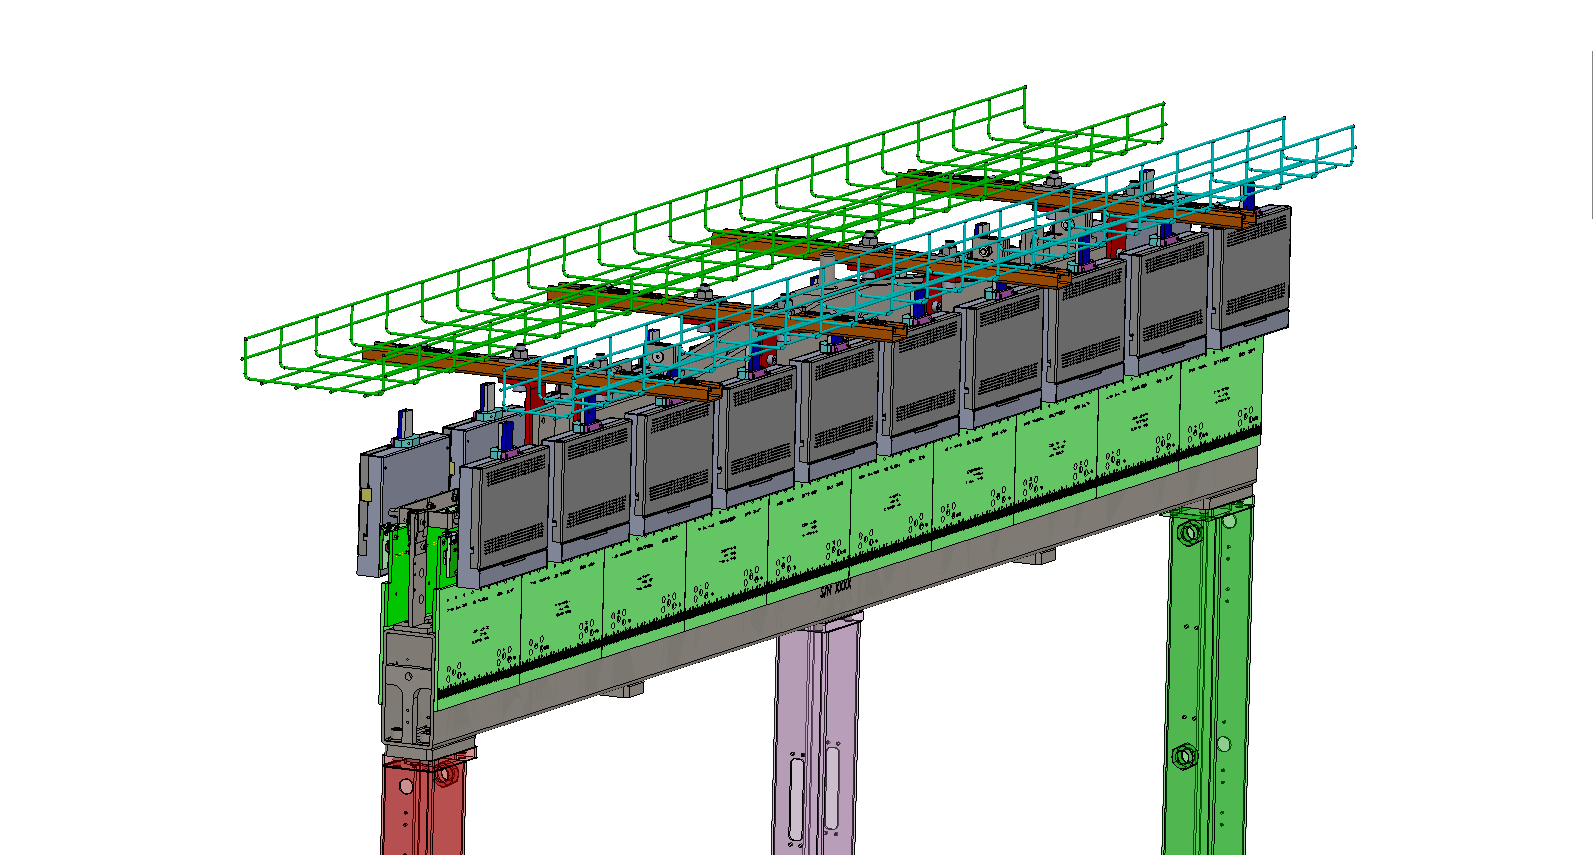
\includegraphics[width=0.8\textwidth]{APA_interface.png}
\end{dunefigure}

The interface between the APA and TPC cold electronics covers a wide range of topics, including the hardware
design and production, testing, integration, installation, and commissioning. The hardware interface basically
has two (mechanical and electrical) components. The mechanical interface includes the support of 20 CE boxes 
with each housing a FEMB. The CE electrical cables need to be routed, so that the head frame of the lower APA
of the 2-APA assembly can be reached. The default design is to rout the CE cables (power and signal) inside the 
two side beams of the APA frame. The electrical interface covers i) the choice of wire-bias voltages to the four 
wire planes, so that 100\% transparency can be achieved for drifting ionization electrons, ii) cable 
connection for the wire bias voltages from the cryostat feedthroughs to the CR boards, iii) interface boards 
providing connection between CR boards and CE boxes, iv) filtering of the wire-bias voltages through CR boards 
in order to suppress potential excess of electronics noise,  and v) overall grounding scheme and electrical 
insulation for each APA. The last item is particularly important in order to reach the designed low 
electronics noise level. 




%%%%%%%%%%%%%%%%%%%%%%%%%%%%%%%%%
\subsection{Photon Detection System}
\label{sec:fdsp-apa-intfc-pds}


%%%%%%%%%%%%%%%%%%%%%%%%%%%%%%%%%
\subsection{High Voltage System}
\label{sec:fdsp-apa-intfc-hv}


%%%%%%%%%%%%%%%%%%%%%%%%%%%%%%%%%
\subsection{LBNF Cryostat and Detector Support Structure}
\label{sec:fdsp-apa-intfc-lbnf-dss}


